\documentclass[notitlepage, hidelinks]{article}
\usepackage{natbib}
\usepackage{graphicx}
\usepackage{enumerate}
\usepackage{geometry}
\usepackage{titlesec}
\usepackage{float}
\usepackage{tabularx}
\usepackage[font=footnotesize,labelfont=bf]{caption}
\usepackage{fancyvrb}
\usepackage[ngerman]{babel}
\usepackage{ifxetex,ifluatex}
\usepackage{etoolbox}
\usepackage[svgnames]{xcolor}
\usepackage{tikz}
\usepackage{xcolor}
\usepackage{multirow}
\usepackage{color, colortbl}
\usepackage{wrapfig}
\usepackage{changepage}
\usepackage{listings}
\usepackage[hyphens]{url}
\usepackage{hyperref}
\usepackage{tikz}
\usepackage{caption}
\newcommand\ytl[2]{
\parbox[b]{16em}{\hfill{\color{black}\bfseries #1}~$\cdots\cdots$~}\makebox[0pt][c]{$\bullet$}\vrule\quad \parbox[c]{14.5cm}{\vspace{10pt}\color{black}\raggedright #2.\\[10pt]}\\[-3pt]
}

\definecolor{Gray}{gray}{0.75}
\definecolor{LightGray}{gray}{0.9}

\definecolor{red}{rgb}{0,0.2,0.701} 
\definecolor{blue}{rgb}{0.023,0.49,0.0117}
\definecolor{green}{rgb}{0,0.8,0}
\definecolor{cyan}{rgb}{0.0,0.38,0.51}
\definecolor{cloudwhite}{rgb}{1, 1, 1}
\definecolor{black}{rgb}{0,0,0}
\definecolor{bluebg}{rgb}{0.05,0.278,0.63}

\lstset{
language=csh,
basicstyle=\footnotesize\ttfamily,
numbers=left,
numberstyle=\tiny,
numbersep=5pt,
tabsize=1,
extendedchars=true,
breaklines=true,
frame=b,
stringstyle=\color{blue}\ttfamily,
showspaces=false,
showtabs=false,
xleftmargin=20pt,
xrightmargin=3pt,
framexleftmargin=17pt,
framexrightmargin=5pt,
framexbottommargin=4pt,
commentstyle=\color{green},
morecomment=[l]{//}, %use comment-line-style!
morecomment=[s]{/*}{*/}, %for multiline comments
showstringspaces=false,
morekeywords={ abstract, event, new, struct,
as, explicit, null, switch,
base, extern, object, this,
bool, false, operator, throw,
break, finally, out, true,
byte, fixed, override, try,
case, float, params, typeof,
catch, for, private, uint,
char, foreach, protected, ulong,
checked, goto, public, unchecked,
class, if, readonly, unsafe,
const, implicit, ref, ushort,
continue, in, return, using,
decimal, int, sbyte, virtual,
default, interface, sealed, volatile,
delegate, internal, short, void,
do, is, sizeof, while,
double, lock, stackalloc,
else, long, static,
enum, namespace, string},
keywordstyle=\color{cyan},
identifierstyle=\color{black},
backgroundcolor=\color{cloudwhite},
}



\DeclareCaptionFont{white}{\color{white}}
\DeclareCaptionFormat{listing}{\colorbox{bluebg}{\parbox{\textwidth}{\hspace{15pt}#1#2#3}}}
\captionsetup[lstlisting]{format=listing,labelfont=white,textfont=white, singlelinecheck=false, margin=0pt, font={bf,footnotesize}}
\lstset{defaultdialect=[Sharp]C}



\setcounter{secnumdepth}{4}
\usetikzlibrary{backgrounds}
\makeatletter

\tikzset{%
  fancy quotes/.style={
    text width=\fq@width pt,
    align=justify,
    inner sep=1em,
    anchor=north west,
    minimum width=\linewidth,
  },
  fancy quotes width/.initial={.8\linewidth},
  fancy quotes marks/.style={
    scale=8,
    text=gray,
    inner sep=0pt,
  },
  fancy quotes opening/.style={
    fancy quotes marks,
  },
  fancy quotes closing/.style={
    fancy quotes marks,
  },
  fancy quotes background/.style={
    show background rectangle,
    inner frame xsep=0pt,
    background rectangle/.style={
      fill=white!25,
      rounded corners,
    },
  }
}

\newenvironment{fancyquotes}[1][]{%
\noindent
\tikzpicture[fancy quotes background]
\node[fancy quotes opening,anchor=north west] (fq@ul) at (0,0) {``};
\tikz@scan@one@point\pgfutil@firstofone(fq@ul.east)
\pgfmathsetmacro{\fq@width}{\linewidth - 2*\pgf@x}
\node[fancy quotes,#1] (fq@txt) at (fq@ul.north west) \bgroup}
{\egroup;
\node[overlay,fancy quotes closing,anchor=east] at (fq@txt.south east) {''};
\endtikzpicture}


\pgfmathsetmacro{\fq@width}{\linewidth - 2*\pgf@x}


\renewcommand{\figurename}{Abb.}
\geometry{left=3cm, right=3cm, bottom=2cm, top=2.5cm}
\titlespacing*{\section}{0pt}{7ex plus 1ex minus .2ex}{4.3ex plus .2ex}
\titlespacing*{\subsection}{0pt}{7ex plus 1ex minus .2ex}{4.3ex plus .2ex}
\setlength\parindent{0pt}
\newcolumntype{L}[1]{>{\raggedright\let\newline\\\arraybackslash\hspace{0pt}}m{#1}}
\def\changemargin#1#2{\list{}{\rightmargin#2\leftmargin#1}\item[]}
\let\endchangemargin=\endlist 


\begin{document}

\mbox{}\\ \mbox{}\\\mbox{}\\ \mbox{}\\\mbox{}\\ \mbox{}\\\mbox{}\\\mbox{}\\
\mbox{}\\\mbox{}\\\mbox{}\\\mbox{}\\\mbox{}\\\mbox{}\\\mbox{}\\\mbox{}\\
\begin{center}
\huge
\textbf{E-Business Architekturen} \\ 
\LARGE
Prüfungsleistung (Gruppenaufgabe) \\
\mbox{}\\
\large
Ergebnisprotokolle der Komplexübungen 1, 2, 3b und 4d im Rahmen der Veranstaltung E-Business Architekturen  \\

\mbox{}\\ \mbox{}\\
\large
vorgelegt am \\
07.05.2023 \\
\mbox{}\\
an der \\
Hochschule für Wirtschaft und Recht Berlin \\
Fachbereich Duales Studium \\
\end{center}

\mbox{}\\ \mbox{}\\\mbox{}\\ \mbox{}\\\mbox{}\\ \mbox{}\\\mbox{}\\ \mbox{}\\\mbox{}\\ \mbox{}\\
\begin{table}[H]
\begin{tabular}{ l l }
von: 
& Robert Neubert \\
& Danny Neupauer \\
& Hannes Roever \\
Fachrichtung: & Wirtschaftsinformatik \\
Studienjahrgang: & WI20C \\
Studienhalbjahr:& Wintersemester 2022/23 \\
Dozent: & Prof. Dr. Andreas Schmietendorf \\
\end{tabular}
\end{table}

\thispagestyle{empty}
\clearpage
\newpage
\tableofcontents
\thispagestyle{empty}
\clearpage

\normalsize
\pagenumbering{arabic}


\section{Einleitung}
lalala\footnote{Vgl. \cite{athey2018impact}, S.5} und sind insofern für komplexe sozialwissenschaftliche Fragestellungen aufgrund des vorhandenen Bias\footnote{Vgl. \cite{miceli2022studying}, S.3ff} \\
lalalala\footnote{Vgl. \cite{blogKorab}, online}

\section{Aufgabe 1: E-Business Grundlagen}

\subsection{Anwendung des Begriffs E-Business}
Was verbinden Sie mit dem Begriff des E-Business? Versuchen Sie die folgenden Aspekte zu berücksichtigen, nennen Sie ggf. weitere.
\begin{itemize}
\item Organisatorische Aspekte
\item Prozessbezogene Aspekte (z.B. Geschäftsprozess)
\item Technologische Aspekte (z.B. Entwicklung \& Betrieb)
\item Gesellschaftliche Implikationen (z.B. Soziologische Aspekte)
\end{itemize}

\subsection{Beziehung zu domänenspezifischen Lösungen}
Welche Beziehungen sehen Sie zu den folgenden Lösungen?
\begin{itemize}
\item Systeme für das e-Learning (z.B. Moodle oder Open HPI)
\item Systeme für das e-Government (z.B. ELSTER oder Fahrzeugzulassung)
\item Systeme für das e–Banking (z.B. Instant Payment)
\item Systeme für das e-Commerce (z.B. Web Shops)
\end{itemize}

\subsection{Ziele und Erwartungen an E-Business Lösungen}
Welche Ziele und Erwartungen verknüpfen Unternehmen und ihre Kunden mit e-Business-Lösungen?
\begin{itemize}
\item Berücksichtigen sie ggf. unterschiedliche Sichten
\item Nennen Sie ihnen bekannte Lösungen (z.B. aus den Praktika)
\item Identifizieren Sie mögliche Vor- und Nachteile
\end{itemize}

\subsection{Eigenschaften von E-Business Softwarearchitekturen}
Über welche Eigenschaften sollten Softwarearchitekturen für e-Business-Lösungen verfügen?
\begin{itemize}
\item Fragen des Kommunikationssystems
\item Verwendete Rechnerinfrastruktur
\item Eigenschaften entwickelter Softwaresysteme
\end{itemize}

\subsection{E-Business im konkreten Unternehmenskontext}
Wie könnte eine Strategie zur Einführung einer e-Business-Architektur in einem Unternehmen ihrer Wahl aussehen?
\begin{itemize}
\item Notwendige Voraussetzungen \& Rahmenbedingungen
\item Auswirkungen auf das Informationsmanagement (CIO)
\item Auswirkungen auf die Entwicklung von Software (Lösungsanbieter)
\item Auswirkungen auf den Betrieb von Software (Rechenzentren)
\item Mehrwertpotentiale für die Kunden und Lieferanten
\end{itemize}

Worin sehen Sie weitere Aspekte eines digitalen Unternehmens, die mit dem Begriff des e-Business nicht erfasst werden?

\section{Aufgabe 2: }

\begin{table}[h]
\centering
\begin{tabular}{|l|l|}
\hline
Zielvariablen & korrelierende Spalten \\ \hline
Kaufpreis     & \begin{tabular}[c]{@{}l@{}}Adresse\\ Grundstücksfläche\\ Wohnfläche\end{tabular} \\ \hline
Miethöhe      & \begin{tabular}[c]{@{}l@{}}Adresse\\ Wohnfläche\\ Zimmeranzahl\\ Heizungstyp\end{tabular} \\ \hline
\end{tabular}
\end{table}

\begin{lstlisting}[language=Python,frame=single,caption=Filtern von nan- und 0-values,label=cone]
df = df.dropna(subset=['obj_lotArea'])
df = df.dropna(subset=['obj_livingSpace'])
df = df.dropna(subset=['obj_purchasePrice'])
df = df.query('obj_lotArea != 0')
df = df.query('obj_livingSpace != 0')
df = df.query('obj_purchasePrice != 0')
\end{lstlisting}

\begin{figure}[H]
\centering
  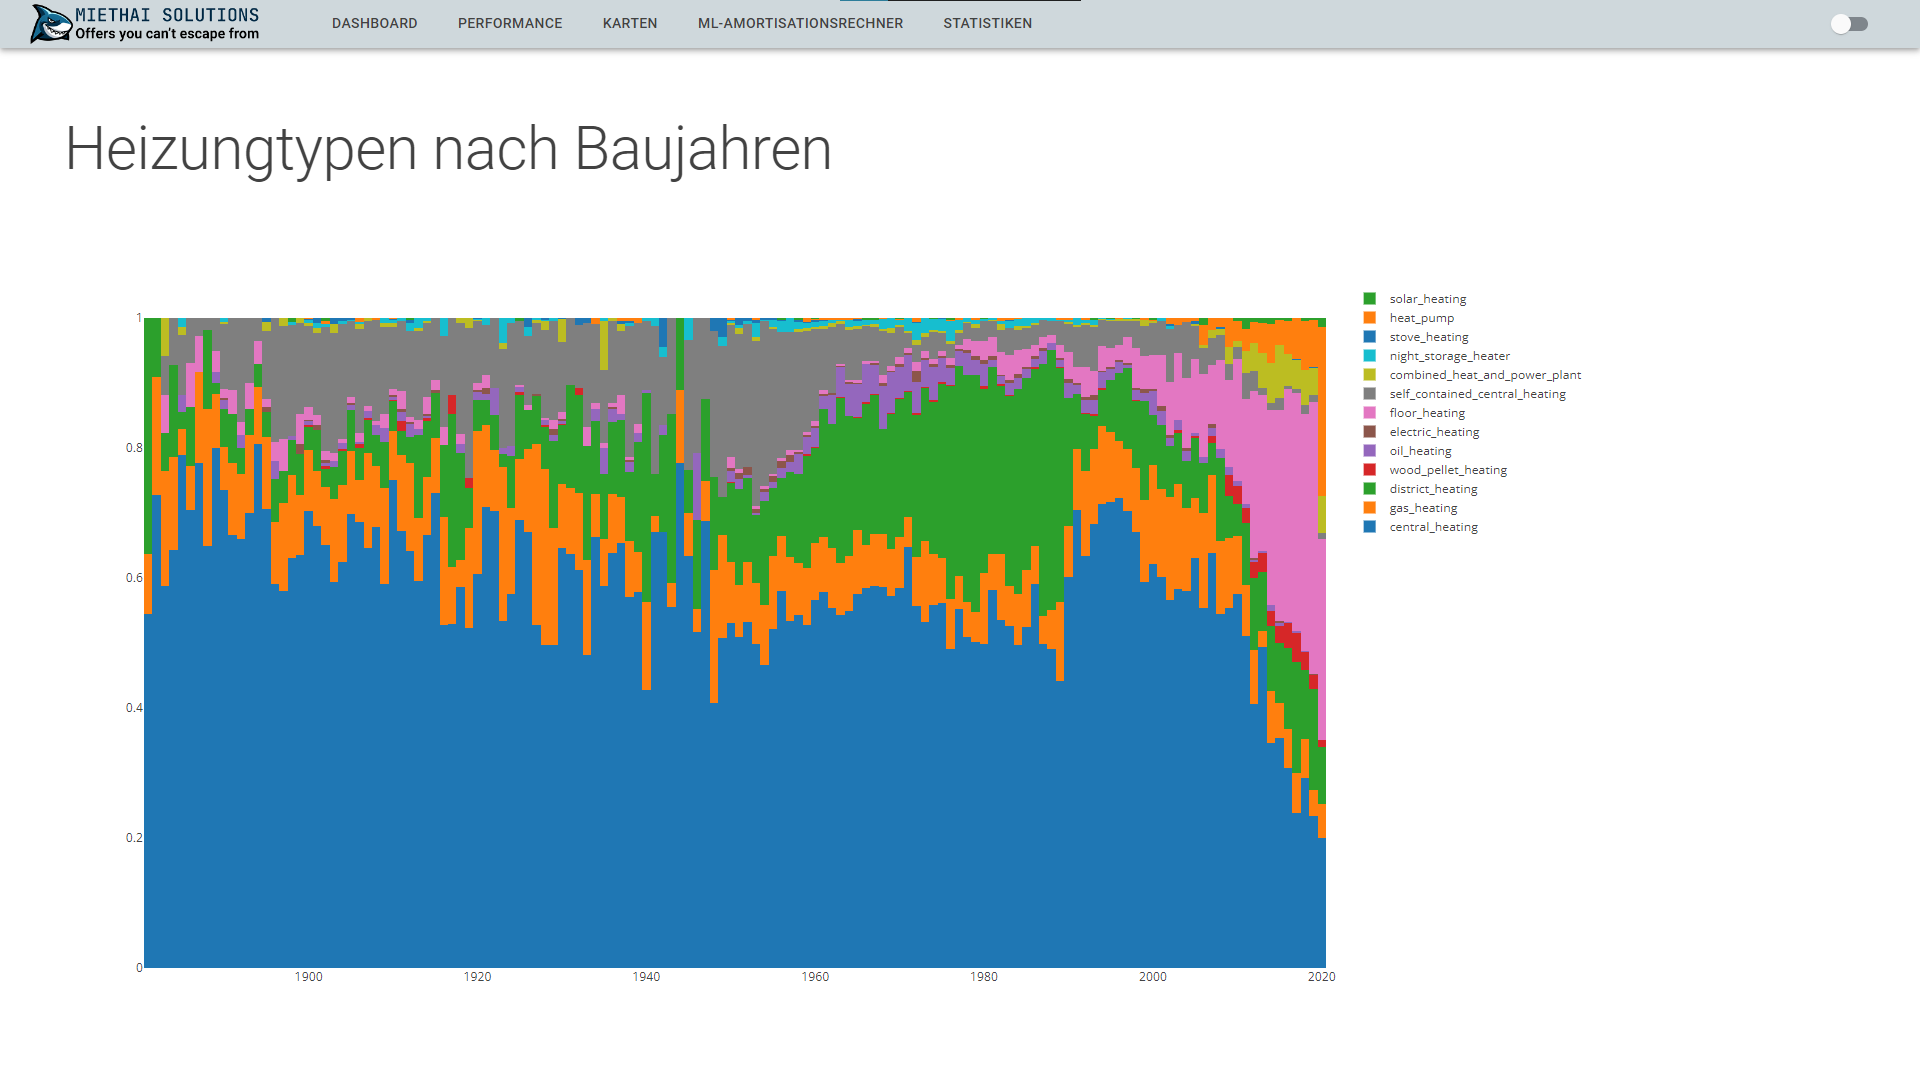
\includegraphics[width=\textwidth]{images/heatingplot.png}
  \caption{Screenshot Heizungsarten Barplot}
  \label{fig:}
\end{figure}

\newpage

\bibliographystyle{te}

\bibliography{citation}

\end{document}